\chapter{Geometrie Non Euclidee}

La teoria che studieremo è una \textit{teoria geometrica}:

\textbf{I 5 postulati di Euclide:}
\begin{enumerate}
    \item Per due qualsiasi punti $A$ e $B$, esiste esattamente una retta che li attraversa.
    \item Una retta può essere prolungata indefinitamente in entrambe le direzioni.
    \item Dato un punto $O$ ed un raggio $R$, esiste esattamente un cerchio con centro in $O$ e raggio $R$.
    \item Tutti gli angoli retti sono congruenti.
    \item Data una retta r ed un punto P fuori da essa, per
    il punto P passa una ed una sola retta parallela ad r (possiamo dare al termine parallelo il significato di \textit{che incontra r solo all'infinito}, in un punto improprio).
\end{enumerate}

Il quinto postulato è più complesso degli altri; i tentativi di dimostrare tale postulato a partire dagli altri postulati, considerati più evidenti, non hanno permesso di arrivare a questo, ma hanno portato, nell'800, alla nascita delle geometrie non-Euclidee (Gauss, Bolyai, Lobachevski, Klein).

\begin{center}
\begin{tikzpicture}[scale=1.0]
    % Draw a dashed line at the top
    \draw[dashed] (-3,1) -- (3,1);
    % Create point P at the center of the dashed line
    \fill (0,1) circle (1pt) node[above] {$P$};
    % Draw the line r at the bottom
    \draw (-3,0) -- (3,0);
    % Place the label r at the left end of the line
    \node at (-2.9,0) [left, above] {$r$};
\end{tikzpicture}
\end{center}

Il quinto postulato si è rivelato indipendente dagli altri enunciati di Euclide, poiché è stato possibile formulare geometrie piane (in 2 dimensioni) in cui valgono tutti gli altri postulati, mentre il concetto di parallelismo assume un significato diverso:

\begin{enumerate}
    \item Non esiste alcuna retta parallela a $R$ passante per $P$ \,\quad $\rightarrow$ \textbf{Geometrie ellittiche piane} $[S^2]$
    \item Esistono due o più rette parallele a $R$ passanti per $P$ \quad $\rightarrow$ \textbf{Geometrie iperboliche piane} $[H^2]$
\end{enumerate}

\begin{figure}[H]
    \centering
    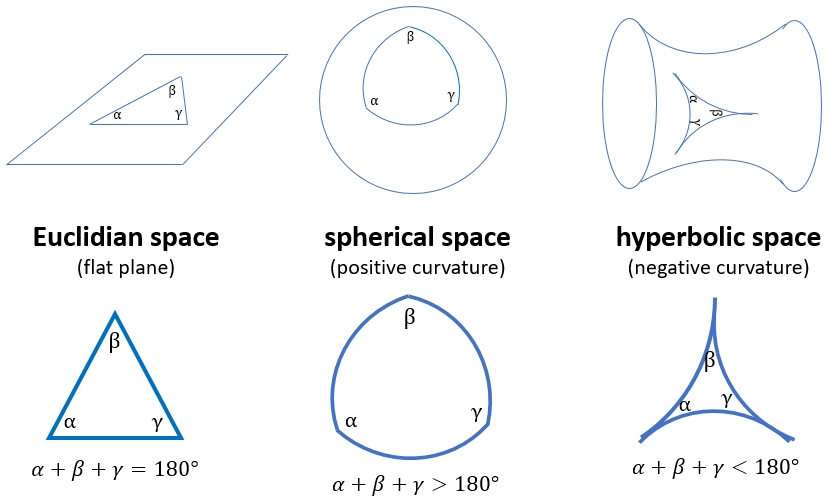
\includegraphics[width=0.6\textwidth]{assets/geometries.png}
    \caption{Geometrie ellittiche e iperboliche}
\end{figure}

\section{Geometria Ellittica}

La \textbf{geometria ellittica piana} è una forma di geometria non euclidea che rifiuta il quinto postulato di Euclide, il quale in geometria euclidea garantisce l'esistenza di una sola retta parallela passante per un dato punto. In geometria ellittica, non esistono rette parallele; invece, ogni coppia di rette si interseca eventualmente.

Un classico esempio è la geometria sferica, in cui possiamo definire come "\bfit{punto}" la coppia di punti diametralmente opposti $(P, P')$, e come "\bfit{retta}" un cerchio massimo passante per $P$ e $P'$. Si può dimostrare che per due punti $(P, P')$ e $(Q, Q')$ passa esattamente una retta $r$. Inoltre, per un punto $(T, T')$ esterno ad $r$ non passa alcuna retta parallela ad $r$, poiché tutte le rette passanti per $(T, T')$ intersecano $r$ in almeno un punto.

Con la geometria analitica, Descartes ha mostrato che, identificando i punti con coppie di numeri reali e definendo la distanza tra due punti $(x_1, y_1)$ e $(x_2, y_2)$ come $d = \sqrt{(x_2 - x_1)^2 + (y_2 - y_1)^2}$, tutti i postulati di Euclide si riducono a teoremi sui numeri reali.

Definito sulla sfera un triangolo con i lati formati da archi di cerchi massimi, la somma degli angoli $\alpha + \beta + \gamma$ è sempre $> \pi$. L'area $S$ di tale triangolo, se la sfera ha raggio $R$, si può esprimere come $S = R^2(\alpha + \beta + \gamma - \pi)$. Quando $S \to 0$ (mantenendo $R$ fisso), si osserva che $(\alpha + \beta + \gamma) \to \pi$. Questo significa che se il triangolo sferico è molto più piccolo del raggio $R$, la sua differenza da un triangolo piano tende a scomparire, avvicinandosi alla geometria euclidea.

\begin{figure}[H]
    \centering
    \begin{minipage}{0.3\textwidth}
        \centering
        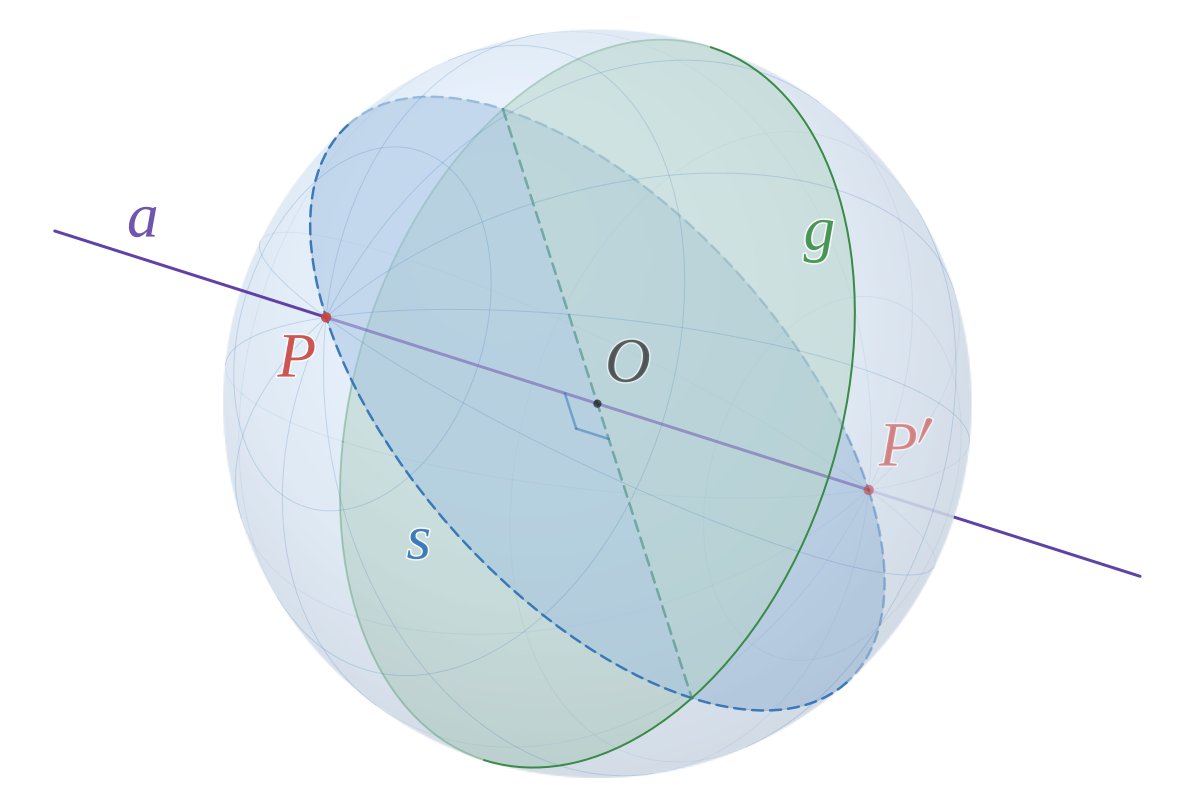
\includegraphics[width=0.85\textwidth]{assets/spherical_geometry.png}
        \caption{Geometria sferica}
    \end{minipage} \hspace{1cm}
    \begin{minipage}{0.3\textwidth}
        \centering
        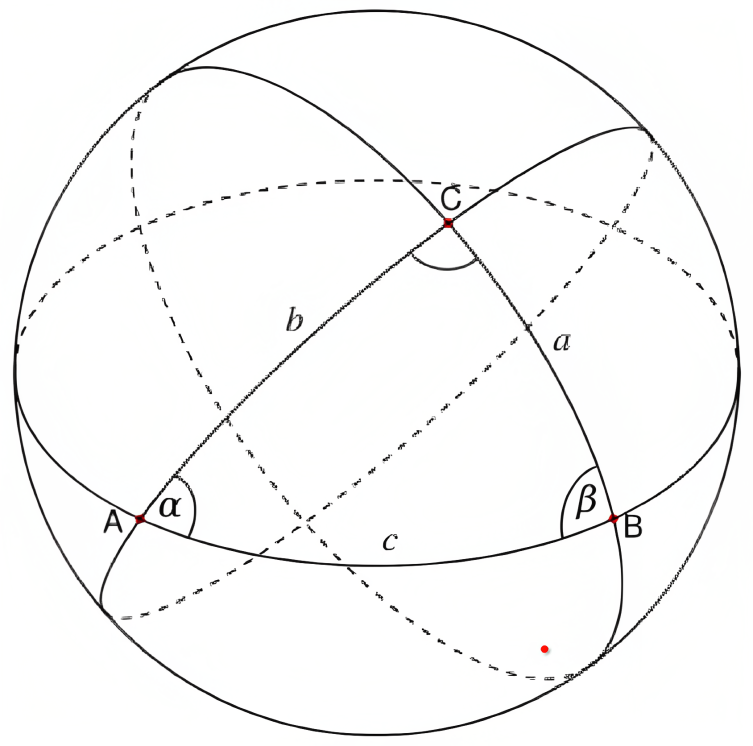
\includegraphics[width=0.82\textwidth]{assets/spherical_triangle.png}
        \caption{Triangolo sferico}
    \end{minipage}
\end{figure}

\vspace{-1em}

In questo contesto, i triangoli, noti come triangoli sferici, mostrano una proprietà intrigante: la somma dei loro angoli interni supera i 180° ($\alpha + \beta + \gamma > \pi$), un fenomeno noto come eccesso sferico, con l'eccesso proporzionale all'area del triangolo.
\vspace{0.2em}
$$
S = R^2(\alpha + \beta + \gamma - \pi) \quad \text{dove per} \quad R \to \infty \quad \text{si ha} \quad \dfrac S{R^2} \to 0 \quad \text{e} \quad \alpha + \beta + \gamma \to \pi
$$
Per costruire un modello della geometria ellittica piana siamo ricorsi all'uso di una sfera (superficie bidimensionale, indicata con $S^2$) immersa (\textit{embedded}) in uno spazio euclideo tridimensionale $E^3$. 

Notiamo che per rappresentare il 5° postulato abbiamo dovuto ricorrere ad una superficie \textit{curva}, cioè la sfera. Questa curvatura deve essere inoltre costante in tutto il piano perché gli altri postulati descrivono lo spazio come omogeneo, e se la curvatura variasse questa proprietà verrebbe meno.

Questo ci porta a comprendere che le diverse geometrie non euclidee possono essere caratterizzate matematicamente attraverso diverse definizioni di distanza. La curvatura dello spazio diventa quindi un elemento fondamentale per distinguere tra i vari tipi di geometrie:
\begin{itemize}
    \item Curvatura zero → geometria euclidea
    \item Curvatura positiva costante → geometria ellittica
    \item Curvatura negativa costante → geometria iperbolica
\end{itemize}

% \begin{figure}[H]
%     \centering
%     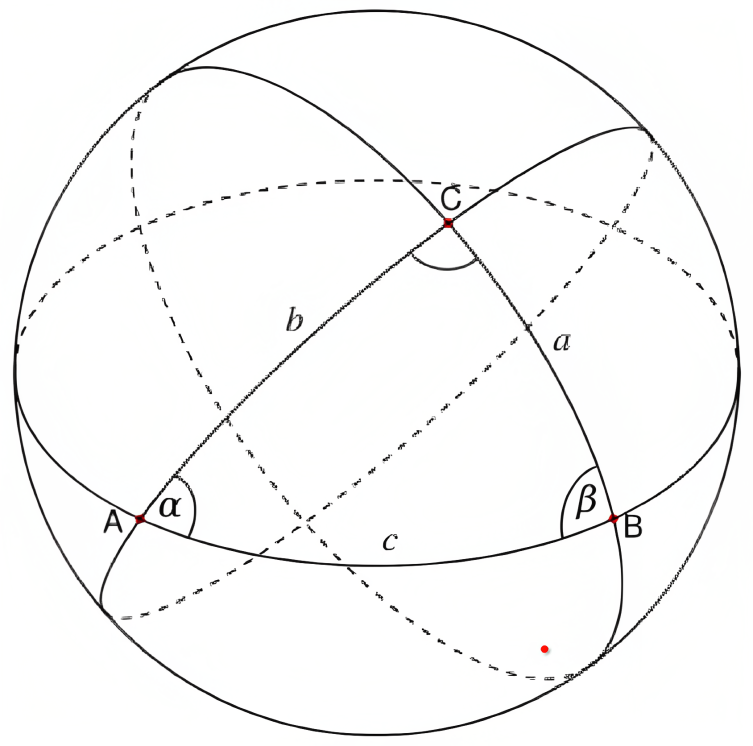
\includegraphics[width=0.4\textwidth]{assets/spherical_triangle.png}
%     \caption{Triangolo sferico}
% \end{figure}

\section{Geometria Iperbolica}

La geometria iperbolica piana è una geometria non euclidea in cui il quinto postulato di Euclide non vale, ammettendo più parallele a una retta data. I triangoli iperbolici hanno somma degli angoli inferiore a 180°, con “difetto” proporzionale all’area. Il piano iperbolico non può essere immerso interamente in uno spazio euclideo 3D, ma esistono modelli come il \emph{cerchio di Klein} (1870), in cui i punti sono all’interno di una circonferenza unitaria e le rette ne sono le corde. Da un punto $P$ passano due parallele a una retta data, e ne esistono infinite che non la intersecano.

\begin{figure}[H]
    \centering
    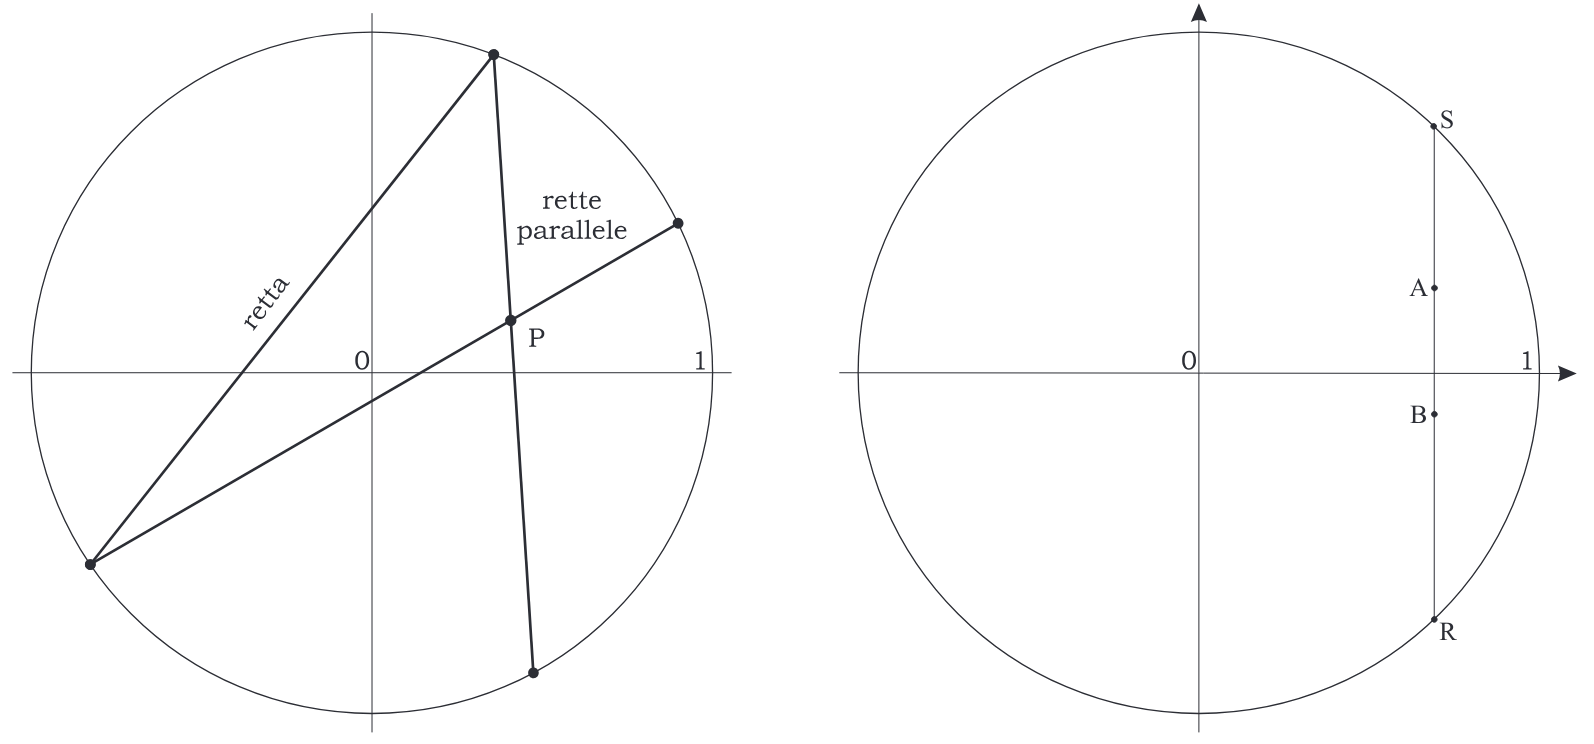
\includegraphics[width=0.75\textwidth]{assets/hyperbolic_geometry.png}
    \caption{Geometria iperbolica}
\end{figure}

La distanza tra due punti $A$ e $B$ è
$$
d(A,B) = \frac12 \log \!\Bigl(\frac{RA\cdot SB}{RB\cdot SA}\Bigr),
$$
che diverge se uno dei punti tende al bordo. Una rappresentazione parziale di $H^2$ in 3D è la \emph{pseudosfera}, una superficie a curvatura negativa costante, in contrasto con la sfera a curvatura positiva.

\section{Curva piana}

Si può parametrizzare una curva piana nel modo seguente: $\bar x(t) = (x_1(t), x_2(t))$, dove $t$ è un parametro, non necessariamente il tempo; il vettore tangente (velocità) è $\tfrac {d\bar x}{dt}$. Possiamo definire l'ascissa curvilinea $s(t)$:
$$
O \equiv \bar x(t = 0) \quad P \equiv \bar x(t) \quad ds = |d\bar x| = |\tfrac {d\bar x}{dt}| dt \quad \to \quad s(t) = \int_0^t |d\bar x| = \int_0^t |\tfrac {d\bar x}{dt}| dt
$$

\begin{figure}[H]
    \centering
    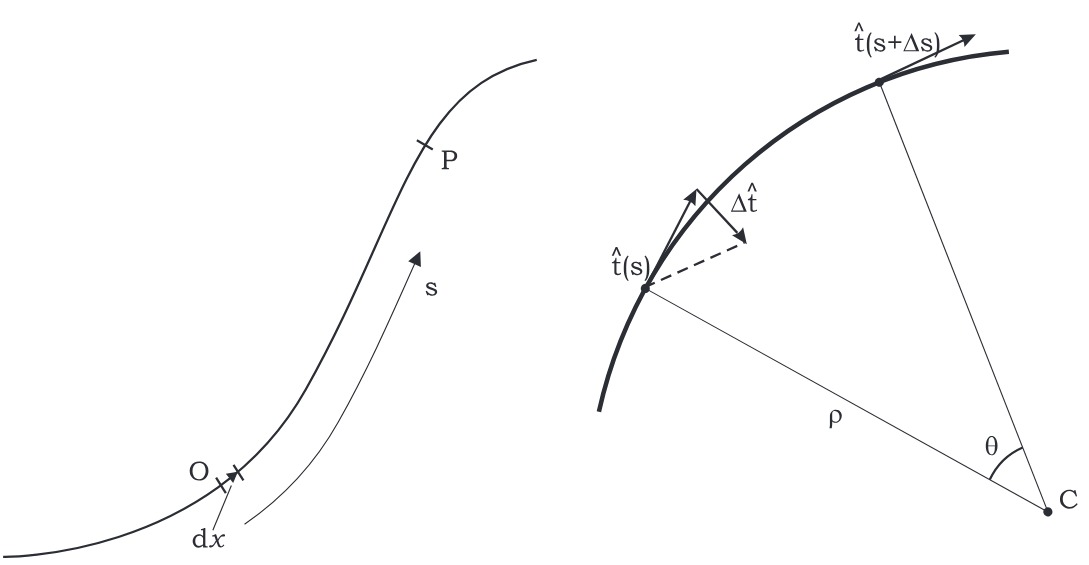
\includegraphics[width=0.5\textwidth]{assets/curve.png}
    \caption{Ascissa curvilinea}
\end{figure}

Trasformando $t \to s$ si può notare che $\dfrac{d\bar x}{ds} = \dot {\bar x}(s)$ ha modulo 1: è il versore tangente $\hat t(s)$.

Poichè $|\dot \bar x(s)| = |\hat t(s)| = 1$, abbiamo $\hat t \dot {\hat t} = 1$ e, derivando, segue che $2 \hat t \cdot \dot {\hat t} = 0$, ovvero $\hat t \perp \dot {\hat t}$.

\textbf{Nota}: $\dot {\hat t}$ non è un versore!

Chiamati $\kappa(s) = |\dot {\hat t}(s)|$ e $\hat n(s) = \dfrac {\dot {\hat t}(s)}{|\dot {\hat t}(s)}$, segue che $\dot {\hat t}(s) = \kappa(s) \hat n(s)$.

$$
\Delta \hat t = \hat t(s + \Delta s) - \hat t(s) 
\quad \quad
|\Delta \hat t| = 2 |\hat t| \sin \dfrac {\Delta \theta}2 \sim \Delta \theta
\quad \quad
\Delta s \simeq \Delta \theta
\quad \quad
\left| \dfrac {\Delta \hat t}{\Delta s} \right| \simeq \dfrac {\Delta \theta}{\rho \Delta \theta} = \dfrac 1\rho
$$

Quindi

$$
\dfrac {d\hat t}{ds} = \kappa\hat n = \dfrac 1\rho \hat n \quad \quad
\begin{cases}
    \kappa : \text{curvatura} \\
    \rho : \text{raggio di curvatura}
\end{cases}
$$

Misurando $\theta$ rispetto ad una distanza fissata (ad esempio la'asse $x$):

$$
\Delta s = \rho \Delta \theta = \dfrac {\Delta \theta}{k} \quad \to \quad \kappa = |\dfrac {d\theta}{ds}|
$$

\begin{figure}[H]
    \centering
    \begin{minipage}{0.3\textwidth}
        \centering
        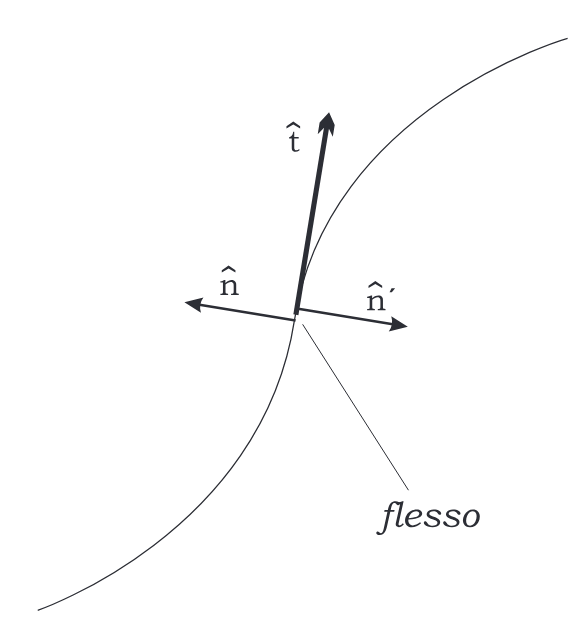
\includegraphics[width=0.95\textwidth]{assets/flesso.png}
        \caption{Curva con flesso}
    \end{minipage}%
    \hspace{10pt}
    \begin{minipage}{0.65\textwidth}
        \centering
        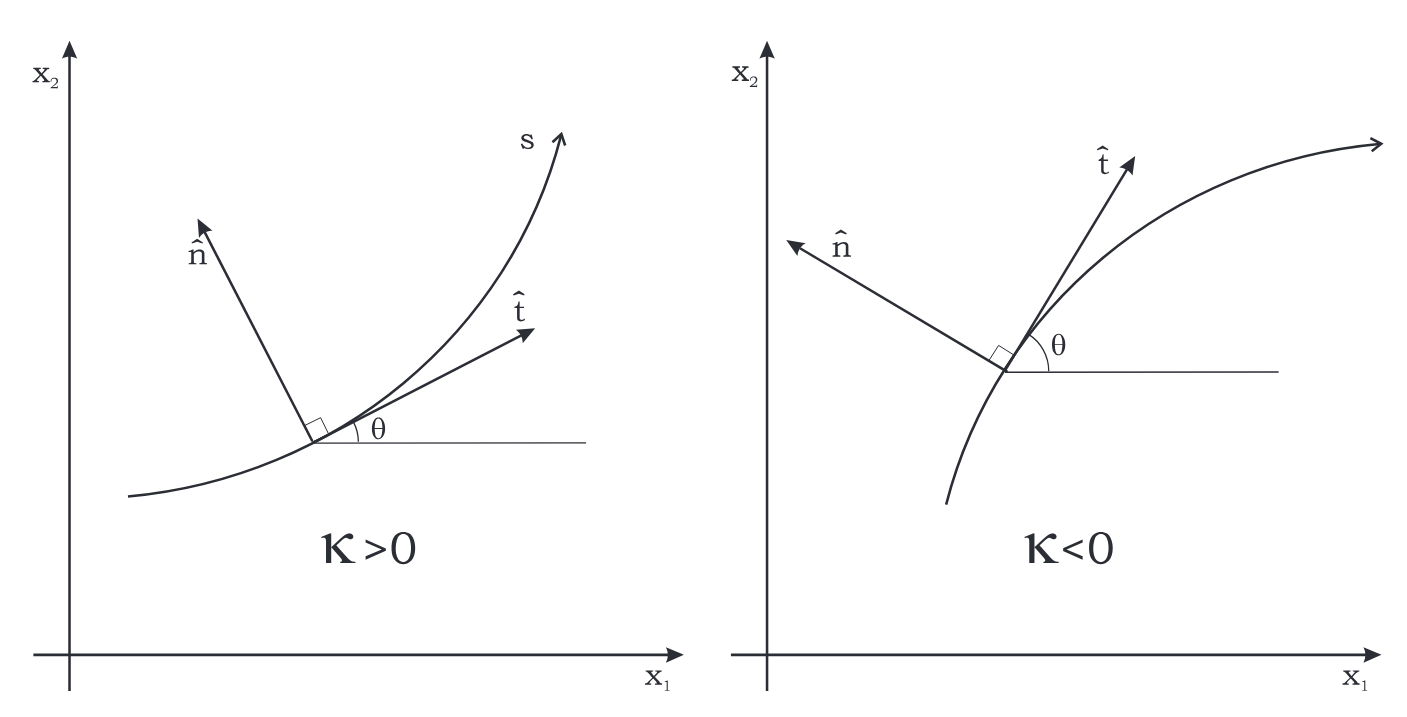
\includegraphics[width=0.95\textwidth]{assets/segno_flesso.png}
        \caption{Segno del flesso}
    \end{minipage}
\end{figure}

Abbiamo definito $\kappa$ come $> 0$. Così facendo, però, in un flesso ho una discontinuità in $\hat n$. Per evitare questo, definita una $s$ sulla curva, resta definito anche $\hat t$ e posso definire $\hat n$ come rotazione di $\hat t$ di 90° in senso positivo (coerente con $O, x_1, x_2$). Poiché $\hat t \perp \dot{\hat t}$ abbiamo ancora $\dot{\hat t} = \kappa\hat n$, ma ora possiamo avere anche $\kappa < 0$. A seconda del segno la curva sta a sinistra o a destra di $\hat t$; nel flesso $\hat n$ non cambia ma $\kappa$ cambia segno e ora risulta:
$$
\kappa = \dfrac {d\theta}{ds}
$$

(e non in valore assoluto).

\section{Superfici}

L'altra volta abbiamo visto come poter usare le coordinate curvilinee per descrivere tre geometrie.
Abbiamo visto poi come 

Ora iniziamo a ragionare con le superfici.

Supponiamo di avere un dominio $D \in \mathbb{R}^2$ e di voler mappare $D$ in un sistema a 3 dimensioni:

$$
\bar{x}(u,v) = (x_1, x_2, x_3) = (x_1(u,v), x_2(u,v), x_3(u,v))
$$

Calcoliamo il gradiente di $\bar{x}$ rispetto a $u$ e $v$:

$$
\begin{cases}
\bar x_u = \frac{\partial \bar x}{\partial u} = \left( \frac{\partial x_1}{\partial u}, \frac{\partial x_2}{\partial u}, \frac{\partial x_3}{\partial u} \right)
\\
\bar x_v =\frac{\partial \bar x}{\partial v} = \left( \frac{\partial x_1}{\partial v}, \frac{\partial x_2}{\partial v}, \frac{\partial x_3}{\partial v} \right)
\end{cases}
$$

Il versore normale alla superficie è dato da:

$$
\hat {n} = \dfrac{\bar x_u \times \bar x_v}{|\bar x_u \times \bar x_v|}
$$

Si dice che la superficie $M$ è regolare (smooth) se il versore normale è ben definito e non nullo, ovvero $\bar x_u$ e $\bar x_v$ non sono paralleli:

$$
\bar x_u \times \bar x_v \neq 0
$$

\subsubsection{Superficie di una sfera di raggio R}

Consideriamo una sfera di raggio $R$ centrata nell'origine. La superficie della sfera è data da:

$$
\bar x(u,v) = (R \cos u \cos v, R \sin u \cos v, R \sin v)
$$
dove $u \in [-\pi, \pi]$, $v \in [-\pi/2, \pi/2]$

\vspace{0.5em}

Calcoliamo il gradiente di $\bar x$ rispetto a $u$ e $v$:

$$
\begin{cases}
\bar x_u = \frac{\partial \bar x}{\partial u} (-R \sin u \cos v, R \cos u \cos v, 0)
\\
\bar x_v = \frac{\partial \bar x}{\partial v} = (-R \cos u \sin v, -R \sin u \sin v, R \cos v)
\end{cases}
$$

Andiamo ad analizzare il punto $(u,v) = (0,0)$:
$$
\begin{cases}
\bar x_u = (0, R, 0)
\\
\bar x_v = (0, 0, R)
\end{cases}
$$

Questi due vettori individuano la superficie tangente alla sfera nel punto $(0,0)$.

Il versore normale alla superficie è dato da:

$$
\hat {n} = \dfrac{\bar x_u \times \bar x_v}{|\bar x_u \times \bar x_v|} = \dfrac{(-R^2, 0, 0)}{R^2} = (-1, 0, 0)
$$

\newpage

\section{Prima Forma Fondamentale}

In geometria differenziale, la \emph{Prima Forma Fondamentale} fornisce la metrica intrinseca di una superficie. Essa permette di calcolare lunghezze, angoli e aree sulla superficie, misurando come essa si deforma nelle diverse direzioni. Consideriamo una superficie liscia parametrizzata da $\bar{x}(u,v)$, dove $u$ e $v$ sono le coordinate locali. I vettori tangenti alla superficie sono definiti da:

$$
\bar{x}_u = \frac{\partial \bar{x}}{\partial u}, \quad \bar{x}_v = \frac{\partial \bar{x}}{\partial v}.
$$

I coefficienti della prima forma sono:

$$
E = \bar{x}_u \cdot \bar{x}_u,\quad F = \bar{x}_u \cdot \bar{x}_v,\quad G = \bar{x}_v \cdot \bar{x}_v.
$$

Un elemento di spostamento infinitesimale sulla superficie si esprime come combinazione lineare dei vettori tangenti. Espandendo il quadrato dello spostamento, otteniamo:

$$
u^2\underbrace{\left(\bar{x}_u \cdot \bar{x}_u\right)}_E + 2uv\underbrace{\left(\bar{x}_u \cdot \bar{x}_v\right)}_F + v^2\underbrace{\left(\bar{x}_v \cdot \bar{x}_v\right)}_G,
$$
da cui il quadrato dell'elemento di lunghezza diventa

$$
ds^2 = E\,du^2 + 2F\,du\,dv + G\,dv^2.
$$

Se una curva sulla superficie è parametrizzata da un parametro $t$, con $u = u(t)$ e $v = v(t)$, allora derivando si ottiene:
$$
\frac{ds^2}{dt^2} = E\, u^2 + 2F\,uv + G\,v^2.
$$

Pertanto, la lunghezza $L$ della curva, per $t$ compreso tra $a$ e $b$, si calcola come:

$$
L = \int_a^b \frac{ds}{dt}\, dt = \int_a^b \sqrt{E\, u^2 + 2F\,uv + G\,v^2}\, dt.
$$

In alternativa, esprimendo direttamente la lunghezza lungo la curva $\bar{r}$ sulla superficie, si ha:

$$
L = \int_{\bar{r}} ds = \int_{\bar{r}} \sqrt{E\,du^2 + 2F\,du\,dv + G\,dv^2}.
$$

Questa formulazione riassume le proprietà geometriche intrinseche della superficie, permettendo di misurare le distanze in maniera indipendente dallo spazio ambiante.


\subsection{Sfera in coordinate sferiche}

Consideriamo una sfera di raggio $R$ centrata nell'origine.La superficie della sfera è data da:

\small
$$
\bar x(u,v) = (R \cos u \cos v, R \sin u \cos v, R \sin v)
\quad \xrightarrow{\text{derive}} \quad
\begin{cases}
    \bar x_u = (-R \sin u \cos v, R \cos u \cos v, 0)
    \\
    \bar x_v = (-R \cos u \sin v, -R \sin u \sin v, R \cos v)
\end{cases}
$$
\normalsize

dove $u \in [-\pi, \pi]$, $v \in [-\pi/2, \pi/2]$

Calcoliamo i coefficienti della prima forma fondamentale:

$$
\begin{cases}
E = \bar{x}_u \cdot \bar{x}_u = R^2 \sin^2 v \cos^2 u + R^2 \sin^2 v \sin^2 u = R^2 \sin^2 v
\\
F = \bar{x}_u \cdot \bar{x}_v = R^2 \sin v \cos v \cos u \cos u + R^2 \sin v \cos v \sin u \sin u = 0
\\
G = \bar{x}_v \cdot \bar{x}_v = R^2 \cos^2 v
\end{cases}
$$

Quindi, la prima forma fondamentale è:

$$
ds^2 = R^2 \sin^2 v\, du^2 + R^2 \cos^2 v\, dv^2
$$

\subsection{Forma metrica}

La forma metrica è una generalizzazione della prima forma fondamentale, che permette di calcolare la lunghezza di curve e la misura di angoli su una superficie. La forma metrica è definita come:

$$
g = E\,du^2 + 2F\,du\,dv + G\,dv^2
$$

dove $E$, $F$ e $G$ sono i coefficienti della prima forma fondamentale. La forma metrica è una forma bilineare simmetrica, che può essere rappresentata da una matrice:

$$
\begin{pmatrix}
    a & b \\
\end{pmatrix}
\underbrace{
\begin{pmatrix}
E & F \\
F & G
\end{pmatrix}
}_{\small \text{Forma metrica}}
\begin{pmatrix}
    c \\
    d
\end{pmatrix}
$$

\subsection{Identità di Lagrange}

L'identità di Lagrange è una relazione che lega la forma metrica e la prima forma fondamentale di una superficie.

$$
\bar x_u \times \bar x_v \neq 0 \quad \Rightarrow \quad \hat N = \dfrac{\bar x_u \times \bar x_v}{|\bar x_u \times \bar x_v|}
$$

L'identità di Lagrange afferma che:

$$
|\bar x_u \times \bar x_v|^2 =
\det
\begin{pmatrix}
    E & F \\
    F & G
\end{pmatrix}
$$

\subsubsection{Dimostrazione}

Iniziamo considerando il prodotto vettoriale tra $\bar x_u$ e $\bar x_v$:

$$
\bar x_u \times \bar x_v = |\bar x_u| |\bar x_v| cos \theta
$$

dove $\theta$ è l'angolo tra $\bar x_u$ e $\bar x_v$. Elevando al quadrato, otteniamo:

$$
|\bar x_u \times \bar x_v|^2 = (|\bar x_u|^2 |\bar x_v|^2 \sin^2 \theta) = |\bar x_u|^2 |\bar x_v|^2 (1 - \cos^2 \theta) = \underbrace{|\bar x_u|^2}_E \cdot \underbrace{|\bar x_v|^2}_G - \underbrace{(\bar x_u \cdot \bar x_v)^2}_{F^2}
$$

Ricordando che $|\bar x_u \times \bar x_v|^2 = \det \begin{pmatrix} E & F \\ F & G \end{pmatrix}$, otteniamo l'identità di Lagrange:

$$
\det \begin{pmatrix} E & F \\ F & G \end{pmatrix} = EG - F^2
$$

\dots

\newpage

$$
g_{ij} = \begin{pmatrix}
    g_{11} & g_{12} \\
    g_{21} & g_{22}
\end{pmatrix}
$$

$$
g_{i,j} = \bar x_i \cdot \bar x_j
$$

$$
\vec v = \sum_i v^i \bar x_i
$$
$$
\vec w = \sum_j w^j \bar x_j = 
$$

forma matriciale tensore metrico

$$
ds^2 = g_{ij} du^i du^j
$$
